\documentclass[ignorenonframetext]{beamer}
%\documentclass[10pt,notes=hide]{beamer}
%\documentclass[10pt,draft,notes=hide]{beamer}

%  \documentclass[ignorenonframetext]{article}
%  \usepackage{beamerarticle}

\usepackage[T1]{fontenc}
\usepackage[utf8x]{inputenc}
\usepackage{inputenc}
\usepackage[magyar]{babel}
\usepackage{ucs}
\usepackage{tabularx}
\usepackage{fancyvrb}

\usepackage{tikz}
\tikzset{ %inner sep = 0.5mm,
  %minimum size = 5mm,
  {future point/.style} ={circle,color=white,draw},%,inner sep=0, minimum size= 1mm}
  point/.style ={circle,draw=black!60,fill=black!20},
   {new point/.style} ={point,fill=blue!30,draw=blue!60},
   {edge/.style} ={thick,draw},
   {new edge/.style} ={draw,thick,-, blue!50},
 }

\mode<article>
{
  \usepackage{fullpage}
  \usepackage{pgf}
  \usepackage[pdftex,colorlinks=true,linkcolor=blue,urlcolor=blue]{hyperref}
  \usepackage{hyperref}
  \usepackage{fancyvrb}
  \setjobnamebeamerversion{python.beamer}
}

\mode<presentation>
{
%  \usetheme{Dresden}
  \usetheme{Warsaw}
%  \usepackage{beamerthemebars}

%  \setbeamercovered{transparent}
}

\newtheorem{definicio}{Definíció}

%pygments-hez
\usepackage{fancyvrb}
\usepackage{color}
\newcommand\at{@}
\newcommand\lb{[}
\newcommand\rb{]}
\newcommand\PYbg[1]{\textcolor[rgb]{0.00,0.50,0.00}{\textbf{#1}}}
\newcommand\PYbf[1]{\textcolor[rgb]{0.73,0.40,0.53}{\textbf{#1}}}
\newcommand\PYbe[1]{\textcolor[rgb]{0.40,0.40,0.40}{#1}}
\newcommand\PYbd[1]{\textcolor[rgb]{0.73,0.13,0.13}{#1}}
\newcommand\PYbc[1]{\textcolor[rgb]{0.00,0.50,0.00}{\textbf{#1}}}
\newcommand\PYbb[1]{\textcolor[rgb]{0.40,0.40,0.40}{#1}}
\newcommand\PYba[1]{\textcolor[rgb]{0.00,0.00,0.50}{\textbf{#1}}}
\newcommand\PYaJ[1]{\textcolor[rgb]{0.73,0.13,0.13}{#1}}
\newcommand\PYaK[1]{\textcolor[rgb]{0.00,0.00,1.00}{#1}}
\newcommand\PYaH[1]{\fcolorbox[rgb]{1.00,0.00,0.00}{1,1,1}{#1}}
\newcommand\PYaI[1]{\textcolor[rgb]{0.69,0.00,0.25}{#1}}
\newcommand\PYaN[1]{\textcolor[rgb]{0.00,0.00,1.00}{\textbf{#1}}}
\newcommand\PYaO[1]{\textcolor[rgb]{0.00,0.00,0.50}{\textbf{#1}}}
\newcommand\PYaL[1]{\textcolor[rgb]{0.73,0.73,0.73}{#1}}
\newcommand\PYaM[1]{\textcolor[rgb]{0.74,0.48,0.00}{#1}}
\newcommand\PYaB[1]{\textcolor[rgb]{0.00,0.25,0.82}{#1}}
\newcommand\PYaC[1]{\textcolor[rgb]{0.67,0.13,1.00}{#1}}
\newcommand\PYaA[1]{\textcolor[rgb]{0.00,0.50,0.00}{#1}}
\newcommand\PYaF[1]{\textcolor[rgb]{1.00,0.00,0.00}{#1}}
\newcommand\PYaG[1]{\textcolor[rgb]{0.10,0.09,0.49}{#1}}
\newcommand\PYaD[1]{\textcolor[rgb]{0.25,0.50,0.50}{\textit{#1}}}
\newcommand\PYaE[1]{\textcolor[rgb]{0.63,0.00,0.00}{#1}}
\newcommand\PYaZ[1]{\textcolor[rgb]{0.00,0.50,0.00}{\textbf{#1}}}
\newcommand\PYaX[1]{\textcolor[rgb]{0.00,0.50,0.00}{#1}}
\newcommand\PYaY[1]{\textcolor[rgb]{0.73,0.13,0.13}{#1}}
\newcommand\PYaR[1]{\textcolor[rgb]{0.10,0.09,0.49}{#1}}
\newcommand\PYaS[1]{\textcolor[rgb]{0.25,0.50,0.50}{\textit{#1}}}
\newcommand\PYaP[1]{\textcolor[rgb]{0.49,0.56,0.16}{#1}}
\newcommand\PYaQ[1]{\textcolor[rgb]{0.40,0.40,0.40}{#1}}
\newcommand\PYaV[1]{\textcolor[rgb]{0.00,0.00,1.00}{\textbf{#1}}}
\newcommand\PYaW[1]{\textcolor[rgb]{0.73,0.13,0.13}{#1}}
\newcommand\PYaT[1]{\textcolor[rgb]{0.50,0.00,0.50}{\textbf{#1}}}
\newcommand\PYaU[1]{\textcolor[rgb]{0.82,0.25,0.23}{\textbf{#1}}}
\newcommand\PYaj[1]{\textcolor[rgb]{0.00,0.50,0.00}{#1}}
\newcommand\PYak[1]{\textcolor[rgb]{0.73,0.40,0.53}{#1}}
\newcommand\PYah[1]{\textcolor[rgb]{0.63,0.63,0.00}{#1}}
\newcommand\PYai[1]{\textcolor[rgb]{0.10,0.09,0.49}{#1}}
\newcommand\PYan[1]{\textcolor[rgb]{0.67,0.13,1.00}{\textbf{#1}}}
\newcommand\PYao[1]{\textcolor[rgb]{0.73,0.40,0.13}{\textbf{#1}}}
\newcommand\PYal[1]{\textcolor[rgb]{0.25,0.50,0.50}{\textit{#1}}}
\newcommand\PYam[1]{\textbf{#1}}
\newcommand\PYab[1]{\textit{#1}}
\newcommand\PYac[1]{\textcolor[rgb]{0.73,0.13,0.13}{#1}}
\newcommand\PYaa[1]{\textcolor[rgb]{0.50,0.50,0.50}{#1}}
\newcommand\PYaf[1]{\textcolor[rgb]{0.25,0.50,0.50}{\textit{#1}}}
\newcommand\PYag[1]{\textcolor[rgb]{0.40,0.40,0.40}{#1}}
\newcommand\PYad[1]{\textcolor[rgb]{0.73,0.13,0.13}{#1}}
\newcommand\PYae[1]{\textcolor[rgb]{0.40,0.40,0.40}{#1}}
\newcommand\PYaz[1]{\textcolor[rgb]{0.00,0.63,0.00}{#1}}
\newcommand\PYax[1]{\textcolor[rgb]{0.60,0.60,0.60}{\textbf{#1}}}
\newcommand\PYay[1]{\textcolor[rgb]{0.00,0.50,0.00}{\textbf{#1}}}
\newcommand\PYar[1]{\textcolor[rgb]{0.10,0.09,0.49}{#1}}
\newcommand\PYas[1]{\textcolor[rgb]{0.73,0.13,0.13}{\textit{#1}}}
\newcommand\PYap[1]{\textcolor[rgb]{0.00,0.50,0.00}{#1}}
\newcommand\PYaq[1]{\textcolor[rgb]{0.53,0.00,0.00}{#1}}
\newcommand\PYav[1]{\textcolor[rgb]{0.00,0.50,0.00}{\textbf{#1}}}
\newcommand\PYaw[1]{\textcolor[rgb]{0.40,0.40,0.40}{#1}}
\newcommand\PYat[1]{\textcolor[rgb]{0.10,0.09,0.49}{#1}}
\newcommand\PYau[1]{\textcolor[rgb]{0.40,0.40,0.40}{#1}}


\author{Horváth Árpád <horvath.arpad@roik.bmf.hu>}
\title[Beamer]{A Beamer használata}
\subtitle{a TikZ csomaggal}
\subject{latex, beamer}
\institute[BMF $\rho$IK]{Budapesti Műszaki Főiskola\\
  Regionális Oktatási és Innovációs Központ (ROIK)\\
  Székesfehérvár}

% Delete this, if you do not want the table of contents to pop up at
% the beginning of each subsection:
\AtBeginSection[]
{
  \begin{frame}<beamer>
    \frametitle{Vázlat}
    \tableofcontents[currentsection]
  \end{frame}
}

\AtBeginSubsection[]
{
  \begin{frame}<beamer>
    \frametitle{Vázlat}
    \tableofcontents[currentsection,currentsubsection]
  \end{frame}
}

\begin{document}


\newlength{\maxheight}
\setlength{\maxheight}{0.63\textwidth}


\begin{frame}
 \maketitle
\end{frame}

\begin{frame}<beamer>
  \frametitle{Vázlat}
  \tableofcontents
\end{frame}

\section{Beamer-alapok}


\begin{frame}[fragile]{A beamerről}
apt-get install latex-beamer

Dokumentáció: \verb|locate beameruserguide|\\[2em]

Mindig a forrást nézzük, mi hogy működik.
\end{frame}

 \subsection[Időzítés]{Listák időzített megjelenítése}


\begin{frame}
  \frametitle{Egymás utáni időzítés}

  Valódi hálózatok:
\begin{itemize}
 \item<+-> ismeretségi hálózat,
 \item<+-> Világháló,
 \item<+-> Internet,
\end{itemize}
\end{frame}

\begin{frame}[<+->]
  \frametitle{Egymás utáni időzítés -- másképp}

A frame környezet opciójába kiemeltük.

\begin{itemize}
 \item ismeretségi hálózat,
 \item Világháló,
 \item Internet,
\end{itemize}
\end{frame}

\begin{frame}
  \frametitle{Egymás utáni időzítés kiemeléssel}
  Ezt nem kell érteni, de használható.

  \begin{itemize}
    \item <+-| alert@+> Hogyan hozhatunk létre véletlen gráfot?
    \item <+-| alert@+> Hogyan bonthatjuk összetevőkre (komponensekre)?
    \item <+-| alert@+> Hogyan vizsgálhatjuk meg, hogy ezek fák-e, vagy
	van-e bennük egy vagy több kör?
  \end{itemize}
\end{frame}

\begin{frame}
  \frametitle{Tetszőleges sorrendű időzítés}

  \begin{itemize}
     \item<1-> látszik: 1-
     \item<2-> látszik: 2-
     \item<-2> látszik: -2
     \item<2-3> látszik: 2-3
     \item<3,5> látszik: 3,5
     \item<4-5> látszik: 4-5
     \item<5> látszik: 5
  \end{itemize}

\end{frame}
\subsection[Verbatim]{Kódok idézése (verbatim)}

\begin{frame}[fragile]
  \frametitle{Verbatim környezet és verb parancs}

A verbatim környezethez és verb parancshoz a fragile opció kell:

\verb|\begin{frame}<beamer>[frame]|

  \begin{enumerate}
    \item Ha nem lenne fent telepítsük a bazaar verziókövető rendszert.\\
    Debian és Ubuntu alatt: \emph{sudo} \verb|apt-get install bzr|
    \item Ha nem saját gépen dolgozunk -- és még nincs -- akkor hozzunk
létre saját könyvtárat, és lépjünk bele:
\begin{verbatim}
mkdir jani
cd jani
\end{verbatim}
  \end{enumerate}
\end{frame}

\begin{frame}[fragile]
  \frametitle{A Verbatim környezet}

A fancyvrb környezettel a nagybetűs Verbatim környezet sokmindenre
képes. A színezést a pygmentize végzi.\\[2em]

\begin{Verbatim}[commandchars=@\[\],
  numbers=left,
  frame=single, label=\framebox{euklidesz.py}]
@PYay[def] @PYaK[Euklidesz](a, b):
    @PYad["]@PYad[ Visszaadja a legnagyobb közös osztót.]@PYad["]
    @PYay[if] a @PYbe[<] b:
        a, b @PYbe[=] b, a 
    
    @PYay[while] b @PYbe[!=] @PYaw[0]:
        a, b @PYbe[=] b, a @PYbe[%] b
        
    @PYay[return] a
\end{Verbatim}
\end{frame}

\subsection{Egyéb}

%\begin{frame}
%  \frametitle{Tételszerű környezetek}
%
%  A tételszerű környezetek más dokumentumosztályban (pl. article) is
%működnek, de itt jobban kiemeltek.
%
%  A fájl elején definiáltuk az alábbi környezetet (newtheorem).
%
%  \begin{definicio}
%  A $p(k)$ \alert{fokszámeloszlás} (degree distribution) egy olyan
%függvény, amely az egyes $k$ fokszámokhoz hozzárendeli azt, hogy egy
%véletlenszerűen kiválasztott csúcs milyen valószínűséggel $k$ fokszámú.
%  \end{definicio}
%\end{frame}

\begin{frame}[fragile,<+->]
  \frametitle{A article dokumentumosztály + article csomag}

  \begin{itemize}
    \item Ezzel lehet nyomtásra alkalmasabb alakot csinálni.
    \item Lásd a \LaTeX-forrás elejét.
    \item A \verb|\begin{frame}<beamer>| kezdetű részek kimaradnak
belőle. Ide lehet például rávezető kérdéseket betenni.
    \item A framek-en kívüli szövegek megjelen(het)nek benne, így a
nyomtatásra alkalmasabb forma alakítható ki.
  \end{itemize}
\end{frame}

\begin{frame}<beamer>[<+->]
  Ez nem lesz látható article osztálynál.
\end{frame}

Ez nem lesz látható a beamer osztálynál.



\section[Ábrák]{Képek és TikZ ábrák beillesztése}
\subsection{includegraphics graphicx csomaggal}

\begin{frame}<beamer>
  \frametitle{Kép beillesztése}
  \includegraphics[width=0.75\textwidth]{Erdos_Renyi_degree_dist.pdf}

 pdflatex: PNG, JPG képek és vektorgrafikus PDF ábrák illeszthetőek be.
\end{frame}

 pdflatex: PNG, JPG képek és vektorgrafikus PDF ábrák illeszthetőek be.

\begin{frame}
  \frametitle{Kép beillesztése}
   szöveg -- 
  \includegraphics[width=0.25\textwidth,angle=90]{Erdos_Renyi_degree_dist.pdf}
   -- szöveg -- 
  \includegraphics[width=0.25\textwidth,angle=45]{Erdos_Renyi_degree_dist.pdf}
   -- szöveg
\end{frame}


\subsection{TikZ}

\begin{frame}[fragile]
  \frametitle{TikZ ábra}

A TikZ ábrához a tikz csomag behívása szükséges. Szép vektorgrafikus
ábrákat illeszthetünk a \LaTeX-fájlba. A létrehozott képet
forgathatjuk, átméretezhetjük, változtathatjuk a vonalvastagságot,
színt.

Dokumentáció: \verb|locate pgfmanual.pdf|


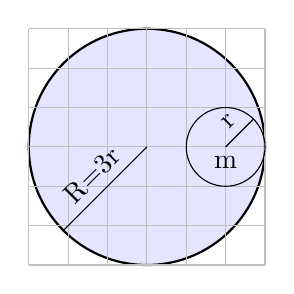
\begin{tikzpicture}[scale=0.5]
\draw[thick,fill=blue!10] (0,0) circle (3);
\draw[color=gray!50] (-3,-3) grid (3,3);
\draw (0,0) -- node[sloped, above]  {R=3r} (225:3);
\draw (2,0) circle (1);
\draw (2,0) -- node[sloped, above]  {r} +(45:1);
\draw (2,0) node[below] {m};
\end{tikzpicture}
\end{frame}

\begin{frame}
  \frametitle{TikZ ábra}

 Szöveget, képletet írhatunk bele a dokumentum betűméretével. Egységes
stílusokat definiálhatunk a a teljes dokumentumra vonatkozóan.


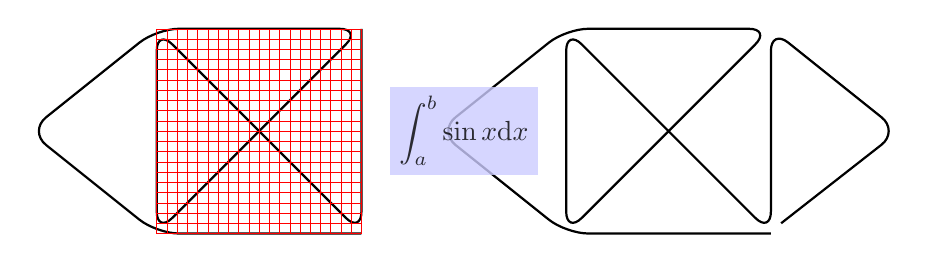
\begin{tikzpicture}[thick, rotate=90, scale=1.3]
\draw[rounded corners=8pt]
  (0,0) -- (0,2) -- (1,3.25) -- (2,2) -- (2,0) -- (0,2) -- (2,2) -- (0,0) -- (2,0);
\draw[rounded corners=8pt]
  ++(0,-4) --  +(0,2) -- +(1,3.25) -- +(2,2) -- +(2,0) -- +(0,2) -- +(2,2) --
+(0,0) -- +(2,0) -- +(1,-1.25) -- +(0.1,-0.1);
\draw[very thin,red,step=1mm] (0,0) grid (2,2);
\node[fill=blue!20,opacity=0.8] (int) at (1,-1) {$\displaystyle\int_a^b \sin x \mathrm d x$};
\end{tikzpicture}
\end{frame}


  Egy TikZ kép részeit is időzíthetjük.

\begin{frame}<beamer>
  \frametitle{Egy TikZ kép részeit is időzíthetjük}

  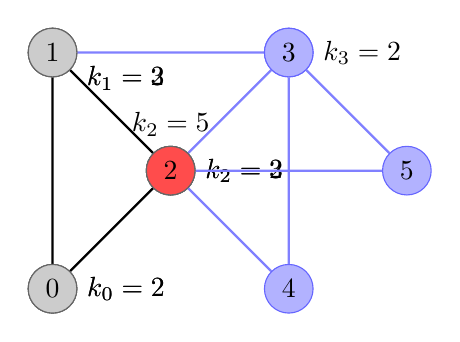
\begin{tikzpicture}[scale=3]
   \node[point] (0) at (0,0) {0};
   \node[point] (1) at (0,1) {1};
   \node[point] (2) at (0.5,0.5) {2};
   \node[future point] (3) at (1,1) {3};
   \node[future point] (4) at (1,0) {4};
   \node[future point] (5) at (1.5,0.5) {5};
   \draw [edge] (0) -- (1) -- (2) -- (0) ;
   \path<2> node[point] at (0) [label=right:{$k_0=2$}] {0};
   \path<2> node[point] at (1) [label=-10:{$k_1=2$}] {1};
   \path<2> node[point] at (2) [label=right:{$k_2=2$}] {2};
   \path<3-> node[new point] at (3) {3};
   \path<3->[new edge] (1) -- (3) -- (2);
   \path<4> node[point] at (0) [label=right:{$k_0=2$}] {0};
   \path<4> node[point] at (1) [label=-10:{$k_1=3$}] {1};
   \path<4> node[point] at (2) [label=right:{$k_2=3$}] {2};
   \path<4> node[new point] at (3) [label=right:{$k_3=2$}] {3};
   \path<5-> node[new point] at (4) {4};
   \path<5->[new edge] (3) -- (4) -- (2);
   \path<6-> node[new point] at (5) {5};
   \path<6->[new edge] (3) -- (5) -- (2);
   \path<7> node[point,fill=red!70] at (2) [label=90:{$k_2=5$}] {2};
  \end{tikzpicture}
  \begin{minipage}{0.48\textwidth}
    \begin{itemize}
      \item<1-> Tetszőleges kicsi hálózatból indulunk.
      \item<2-> A fokszámmal arányos valószínűséggel csatlakozok.
            Kezdetben mindegyiknél $2/6$.
      \item<3-> Itt minden lépésben $m=2$ éllel csatolom az új éleket.
      \item<7> Kialakulnak \alert{nagy fokszámú csúcsok}.
      \item<7> A korán jövőknek előnyük van.
    \end{itemize}
  \end{minipage}
\end{frame}

\begin{frame}
  \tableofcontents
\end{frame}

%%%%%%%%% Vigyázz! Vége következik. %%%%%%%%%%
\end{document}
